
\section{Entr\'{e}e}\label{entree}

%********************************************************************************

\subsection{Portalseite}

Stichworte f"ur die Portalseite der Mumie sind: 

\begin{list_sabina}
\item
\textbf{Design/Graphik:} ansprechend, sch"on, professionell\\
"Ubersicht "uber Haupttools, wenige Buttons
\item
\textbf{Stimmung:} Universalit"at der Mathematik, multikulturell
\item
\textbf{Performance:} kurze Ladezeiten, Lauff"ahigkeit unter bel.
Browsers mu"s mindestens f"ur die Portalseite (und die direkt auf sie
folgenden, eher organisatorisch orientierten Seiten) absolut
sichergestellt sein
\item
\textbf{Inhalt:} Projektname ``Mumie'', Integration der tragenden 
Charaktere (Begleiter), Haupttools, Links (s. unter ``Funktionalit"at'')
\item
\textbf{Funktionalit"at:} Zugang zu
        \begin{sub_list_sabina}
        \item
        Vollversion (mit Authentifizierung) und Demoversion
        \item
        Helppages
        \item
        Infopages
        \item
        Direktzugang zu Haupttools (nachgeschaltete Authentifizierung)
        \end{sub_list_sabina}
\end{list_sabina}

\begin{figure}[h]
\begin{center}
\ifx\pdfoutput\undefined
  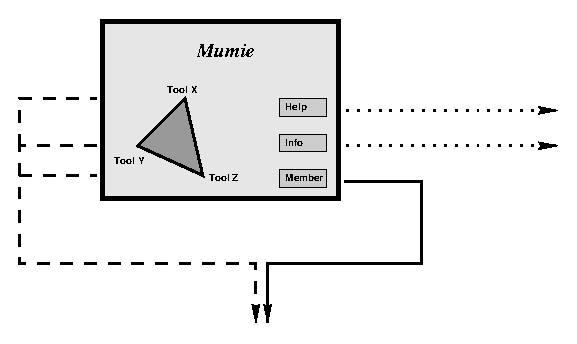
\epsfig{file=Skizzen/portal_main.eps}
\else
  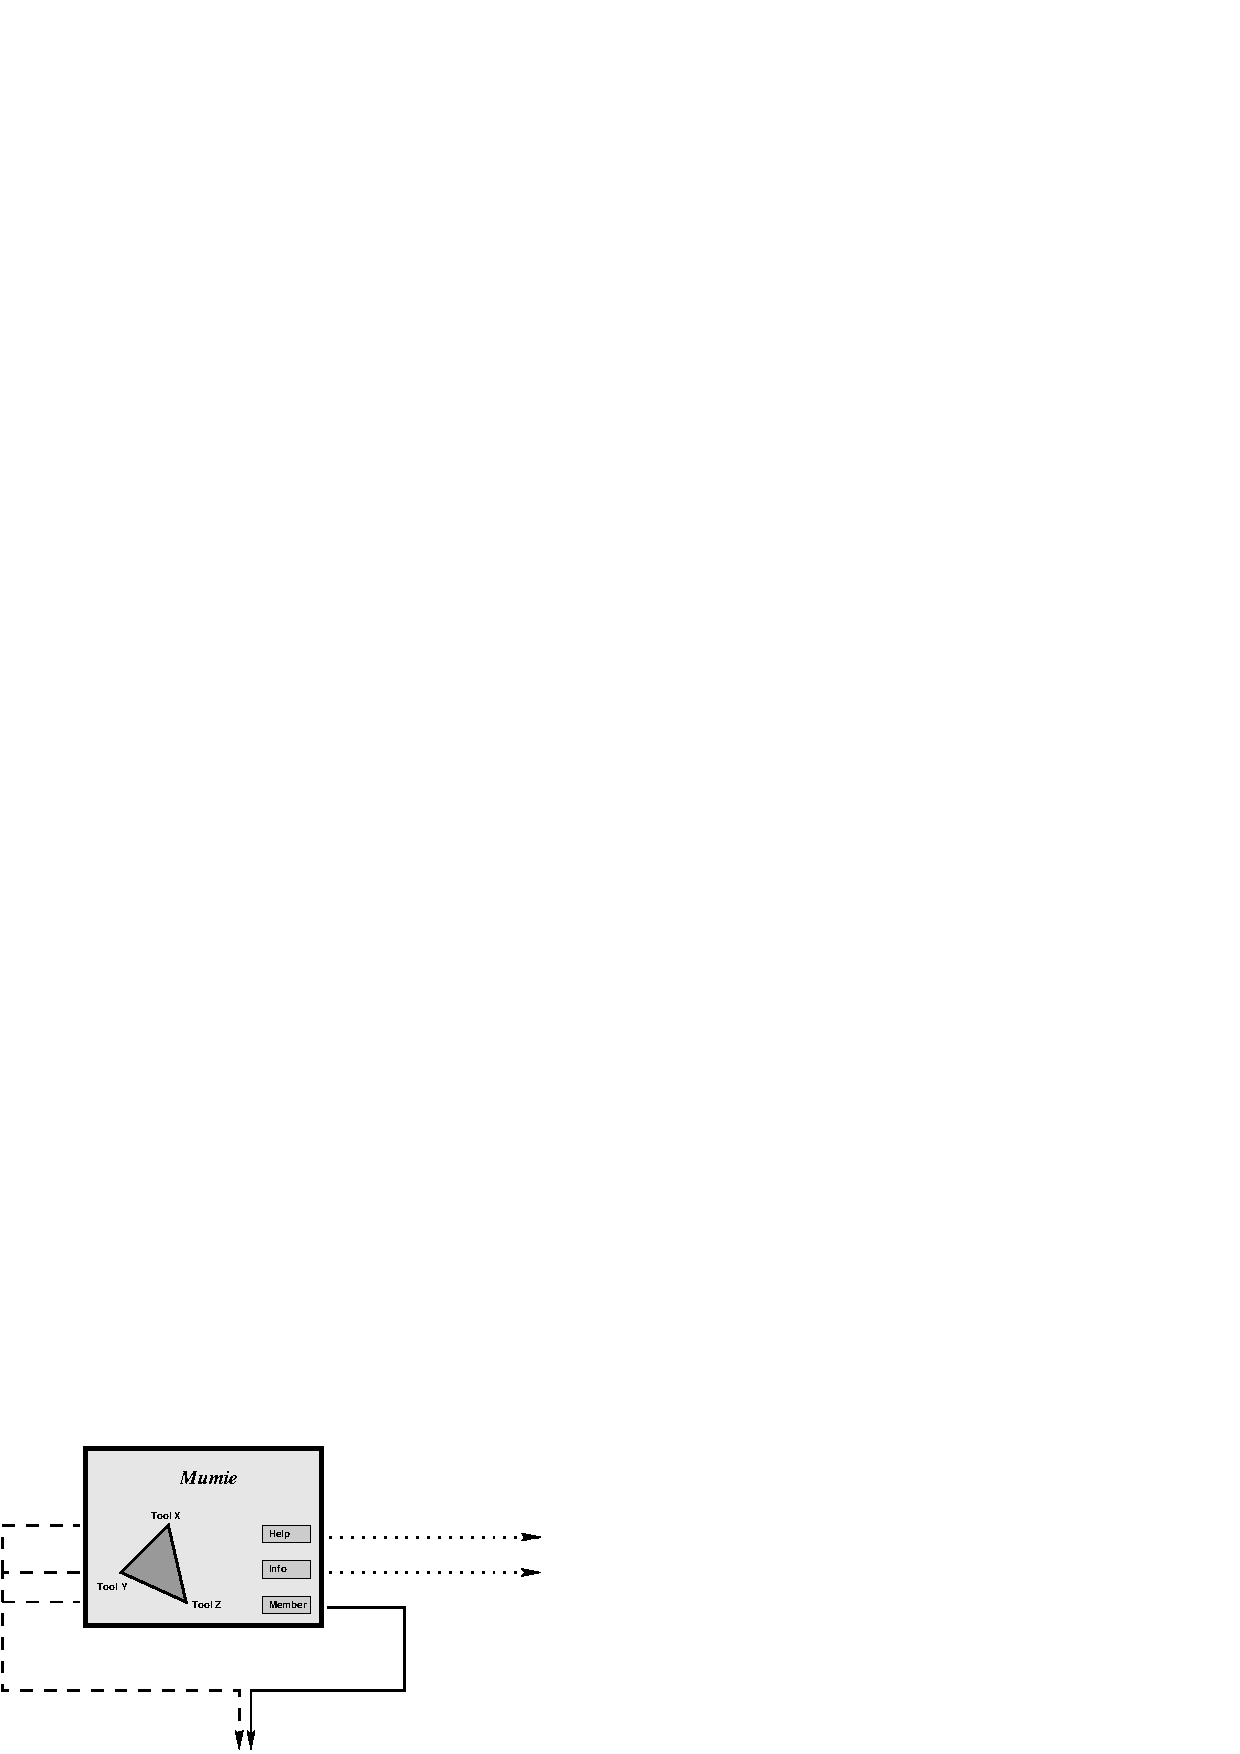
\includegraphics{Skizzen/portal_main.pdf}
\fi
\caption{"Ubersicht "uber das Portal und die direkten Folgeseiten}
\end{center}
\end{figure}
 
Die Logos der beteiligten ProjektPartner-Universit"aten k"onnen,
m"ussen aber nicht unbedingt Bestandteil der Einstiegsseite sein,
zumal etliche andere Verbundprojekte auch davon Abstand nehmen und
sich diese Informationen au"serdem unter direkt von der Portalseite
aus zu erreichenden den Infopages (Kap. \ref{kap:info_pages}) sogar
wesentlich detaillierter pr"asentieren. Hier sollte zun"achst
R"ucksicht auf die graphische Gesamtgestaltung genommen werden.

%********************************************************************************

\clearpage

%********************************************************************************

\subsection{Zug"ange}

Es werden grunds"atzlich zwei Zugangsformen vorgesehen: die ``Vollversion''
(mit Authentifizierung) und eine sog. ``Demoversion''\footnote{Die Demoversion
  beinhaltet einige besonders ansprechende und gelungene Beispiele aus dem
  Projekt und verweist weiter auf die Authentifizierungsseite.  Der Demozugang
  wird vorl"aufig \textit{ohne Inhalte} als Dummy-Zugang realisiert.} (ohne
Identifikation oder
Authentifizierung).

Beide Zugangsformen werden von der Portalseite aus "uber zwei verschiedene
Wege erreicht:
\begin{list_sabina}
\item
\textbf{"uber den Memberbutton} 
\item
\textbf{"uber das Anklicken eines Tools} 
\end{list_sabina}


\subsubsection{Zugang "uber Memberbutton}

Der Usert wird zu einer dreigeteilten Authentifizierungsseite geleitet
(frames; da die einzelnen Teile noch in anderen Kontexten Anwendung finden
k"onnen):

\begin{list_sabina}
\item
\textbf{Authentifizierungsbereich:} (in Skizzen rechts oben)\\
Userid und password werden abgefragt, der Demozugang wird "uber userid
``demo'', password ``demo'' erreicht (dazu existiert ein
erl"auternder Text auf der Seite).
\item
\textbf{Anmeldebereich:} (in Skizzen rechts unten)\\
Liegt (noch) kein userid/password vor, so kann hier ein
solcher Zugang beantragt werden\footnote{Die Vergabe eines Zuganges
erfolgt \textit{nicht} automatisch, sondern durch einen
``Mumienadministrator''.}. Der Neu-User wird zu einer Formular-Seite
geleitet (notwendige Angaben t.b.s.); diese enth"alt die "ublichen
Fehlerabfragen und Best"atigungen beim Absenden.\\
Dieser Bereich beeinhaltet ebenfalls einen erl"auternden Text zu den
grunds"atzlichen Regelungen und Grundlagen f"ur die Vergabe von Zug"angen.
\item
\textbf{Orientierungsbereich:} (in Skizzen links)\\
Der Orientierungsbereich wird i.w. nur mit ansprechender Graphik gestaltet.\\
(Die eigentliche Bedeutung erh"alt dieser Bereich erst beim Zugang
"uber eines der Tools, siehe Kap. \ref{kap:toolzugang}.) 
\end{list_sabina}

\begin{figure}[h!]
\begin{center}
\ifx\pdfoutput\undefined
  \epsfig{file=Skizzen/authent_page_member.eps}
\else
  \includegraphics{Skizzen/authent_page_member.pdf}
\fi
\caption{Authentifizierung "uber den Memberbutton}
\end{center}
\end{figure}



Bei erfolgreichem login erh"alt der User eine Auswahl:

\begin{list_sabina}
\item
\textbf{zur einer zentralen Einstiegs-"Ubersichtsseite der Mumie}\\
(Default nach Demo-Zugang)
        \begin{sub_list_sabina}
        \item
        Zugang zu Haupttools
        \item
        Zugang zum Userprofil
        \end{sub_list_sabina}
\item
\textbf{zur Startseite}
        \begin{sub_list_sabina}
        \item
        des Lerntools
        \item
        des "Ubungstools
        \item
        ...
        \end{sub_list_sabina}
\item
\textbf{zur"uck zur letzten besuchten Seite} (user-spezifisch)
        \begin{sub_list_sabina}
        \item  
        global
        \item
        des Lerntools
        \item
        des "Ubungstools
        \item
        ...
        \end{sub_list_sabina}
\item
\textbf{zu meinem User-Profil}\\
(to be specified)
\end{list_sabina}

\begin{figure}[h!]
\begin{center}
\ifx\pdfoutput\undefined
  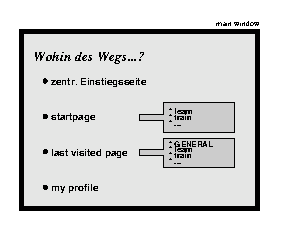
\epsfig{file=Skizzen/weg_auswahl.eps}
\else
  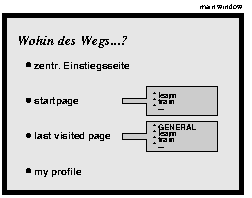
\includegraphics{Skizzen/weg_auswahl.pdf}
\fi
\caption{Auswahl nach erfolgreicher Authentifizierung bei Verwendung
des Memberbuttons}
\end{center}
\end{figure}


\clearpage

\subsubsection{Direktzugang "uber ein Tool}\label{kap:toolzugang}

Es werden nur die Unterschiede zum Zugang "uber den Memberbutton skizziert:

Der Usert wird zu wieder zu der dreigeteilten Authentifizierungsseite
geleitet; der Orientierungsbereich enth"alt nun ein ``Abstract'' aus Graphik
und Text zu dem Tool, das er gew"ahlt hat.

Bei erfolgreichem login erh"alt der User keine weitere Auswahl, sondern wird
direkt auf die letzte besuchte Seite des Tools geleitet, das er angew"ahlt
hat.  Damit erreicht er diesen Punkt nach nur \textit{einem} Zwischenschritt
(der Authentifizierung, die nicht eingespart werden kann).

\begin{figure}[h]
\begin{center}
\ifx\pdfoutput\undefined
  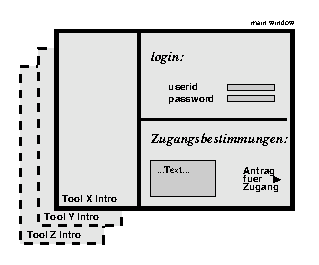
\epsfig{file=Skizzen/authent_page_tool.eps}
\else
  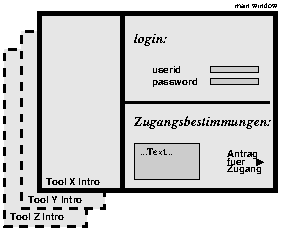
\includegraphics{Skizzen/authent_page_tool.pdf}
\fi
\caption{Authentifizierung "uber ein Tool}
\end{center}
\end{figure}


\subsubsection{Fehlermeldung bei der Authentifizierung}

Bei nicht-erfolgreichem login erh"alt der User eine entsprechende
Fehlermeldung sowie erneute Einlog-M"oglichkeit (die urspr"ungliche
Authentifizierungsseite erscheint wieder, erg"anzt um die
Fehlermeldung und Erl"auterungen, Link zur Kontaktaufnahme mit dem
Webmaster etc.).

\begin{figure}[h]
\begin{center}
\ifx\pdfoutput\undefined
  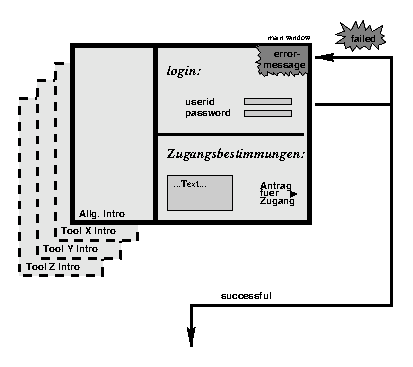
\epsfig{file=Skizzen/authent_page_error.eps}
\else
  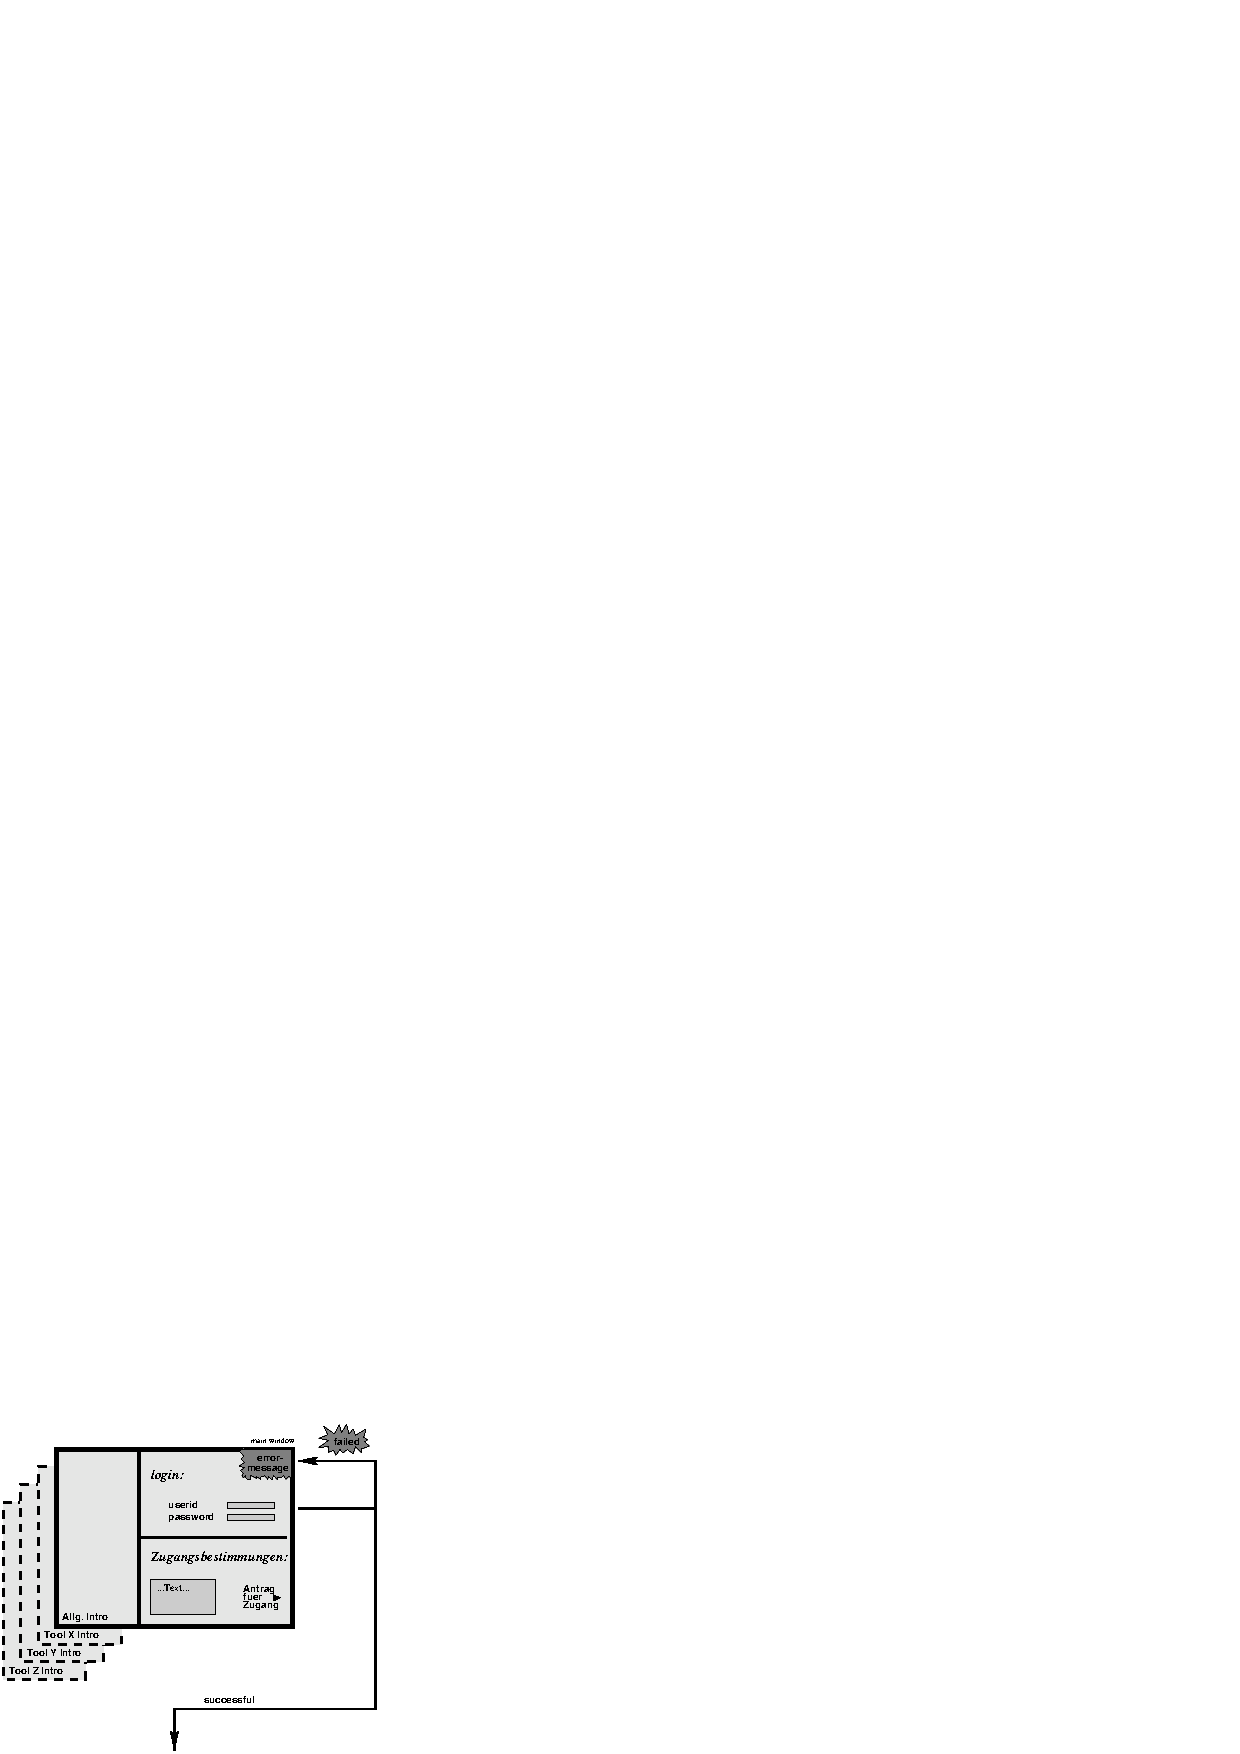
\includegraphics{Skizzen/authent_page_error.pdf}
\fi
\caption{Fehlermeldung bei Authentifizierung "uber Memberbutton \textit{und} Tool}
\end{center}
\end{figure}

\clearpage

\subsubsection{Graphische "Ubersicht "uber die Zug"ange}

\begin{figure}[h!]
\begin{center}
\ifx\pdfoutput\undefined
  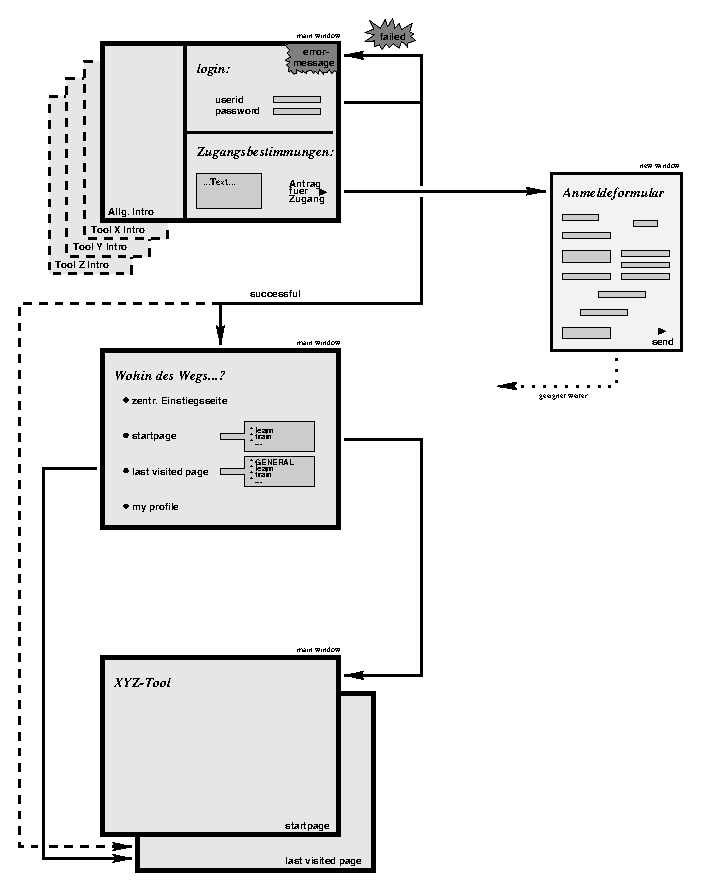
\epsfig{file=Skizzen/authent_page_overview.eps}
\else
  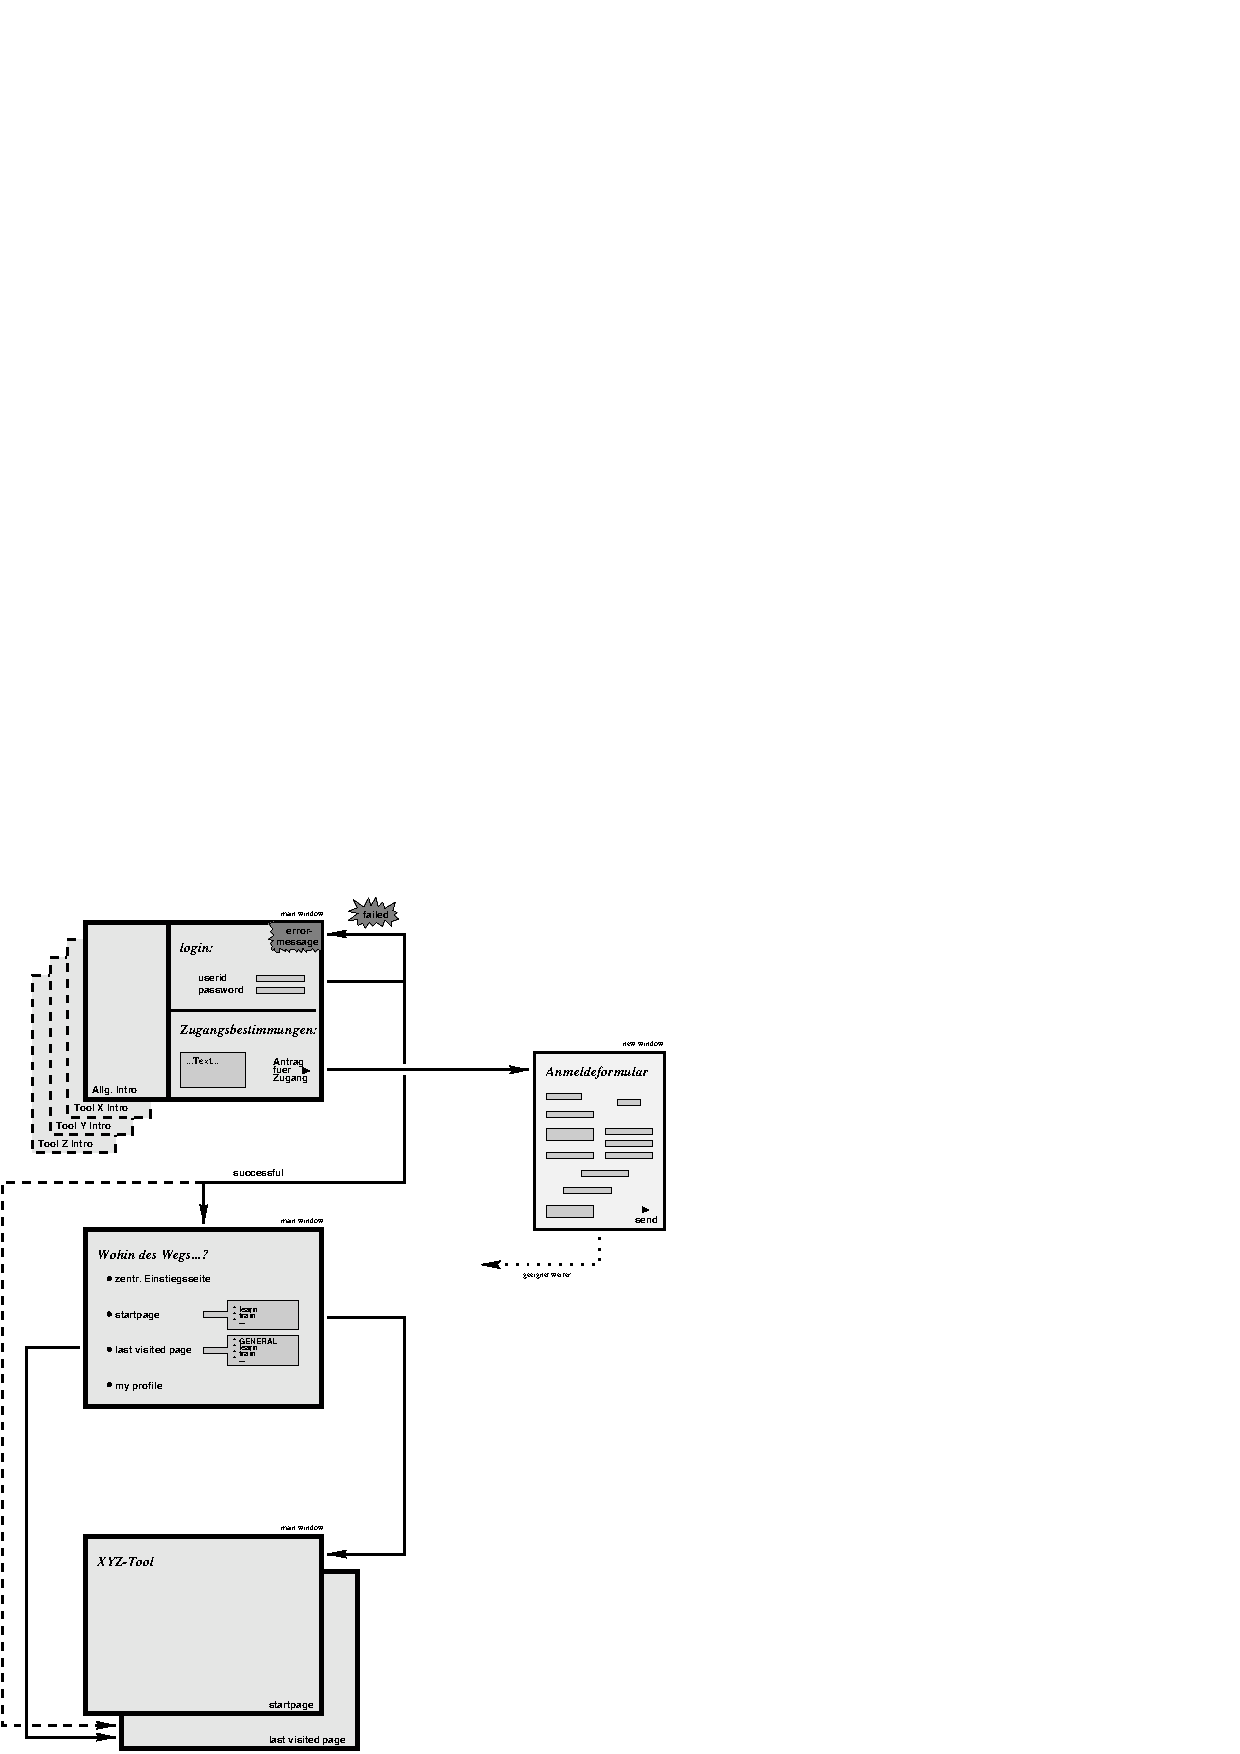
\includegraphics{Skizzen/authent_page_overview.pdf}
\fi
\caption{Authentifizierung "uber Memberbutton \textit{und} Tool}
\end{center}
\end{figure}
 
%********************************************************************************

\clearpage

%********************************************************************************

\subsection{Help-Pages}

Die Help-Pages werden an die graphisch-thematische Idee der Einstiegsseite 
angelehnt.\\
Sie zerfallen in folgende Bereiche:

\begin{list_sabina}
\item
\textbf{"Ubersichtsseiten:}
Die oberste Hierarchie der Help-Pages gibt eine "Ubersicht in die
gesamte Lernsoftware ``Mumie'', insbesondere "uber
die bestehenden Tools und deren Zusammenh"ange.
\item
\textbf{Toolspezifische Seiten:}
Die zentralen Teile der Help-Pages sind toolspezifisch und werden daher erst
mit fortschreitender Entwicklung der Tool differenziert beschrieben.
\item
\textbf{Seiten f"ur externe Helferlein:}
Der Einstieg eventuell angeschlossener/integrierter Tools (wie MathLab,
Mathematica, ...) und anderer potentiell sinnvoller Erg"anzungen
(Programmiersprachen, ...) wird durch (kurze) Dokumentationen unterst"utzt.
\end{list_sabina}

Bei den Help-Pages mu"s sorgf"altig zwischen ``organisatorischen'' und
``fachlichen'' Anwendungen unterschieden werden.

\vspace{10mm}

t.b.s. in detail

%********************************************************************************

\clearpage

%********************************************************************************

\subsection{Info-Pages}\label{kap:info_pages}

Die Info-Pages zerfallen in folgende Bereiche:

\begin{list_sabina}
\item
\textbf{Allgemeine Informationen:}
F"orderung, wer, wann, was, aktueller Stand, geplante Ausbaustufen, ...
\item
\textbf{Links zu beteiligten Partnern:}
Links zu den Universit"aten, zu den lokalen Projektleiterern, 
zu den Mitarbeitern, ...
\item
\textbf{Hintergrundinfos:}
Artikel etc.
\end{list_sabina}

\vspace{10mm}

t.b.s. in detail

%********************************************************************************

\clearpage

%********************************************************************************

\subsection{Graphische "Ubersicht Entr\'{e}e-Bereich}

%Die skizzierten Zugangswege sind die ``kanonischen''.\\
%Zus"atzlich werden, um der Nichtlinearit"at des Mediums
%und den verschiedenen Userbed"urfnissen gerecht zu werden,
%``quer verlaufende'' zus"atzlich (i.w. aber ohne gro"sen
%Zusatzaufwand) realisiert:

\begin{figure}[h!]
\begin{center}
\ifx\pdfoutput\undefined
  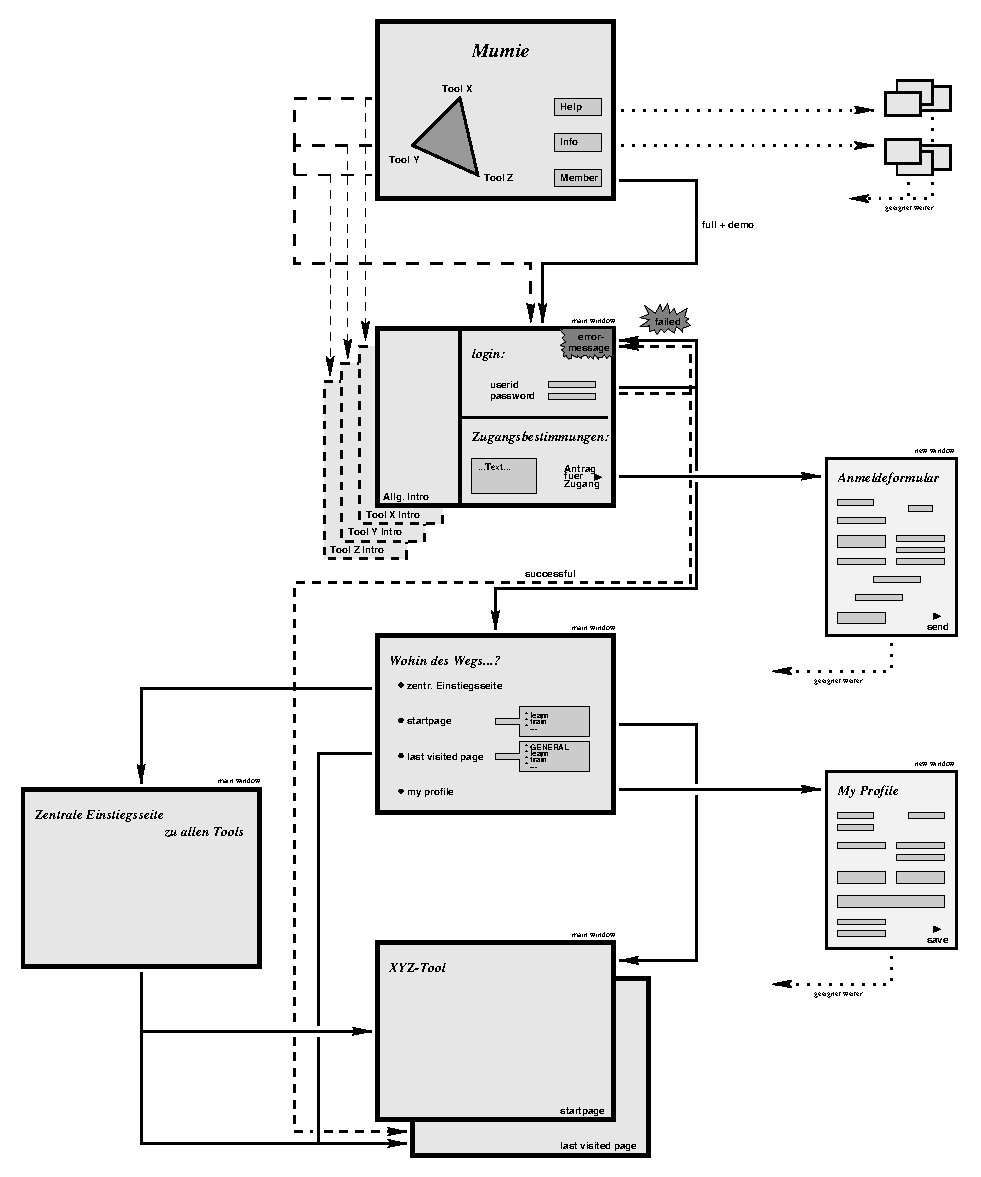
\epsfig{file=Skizzen/overview_portal.eps}
\else
  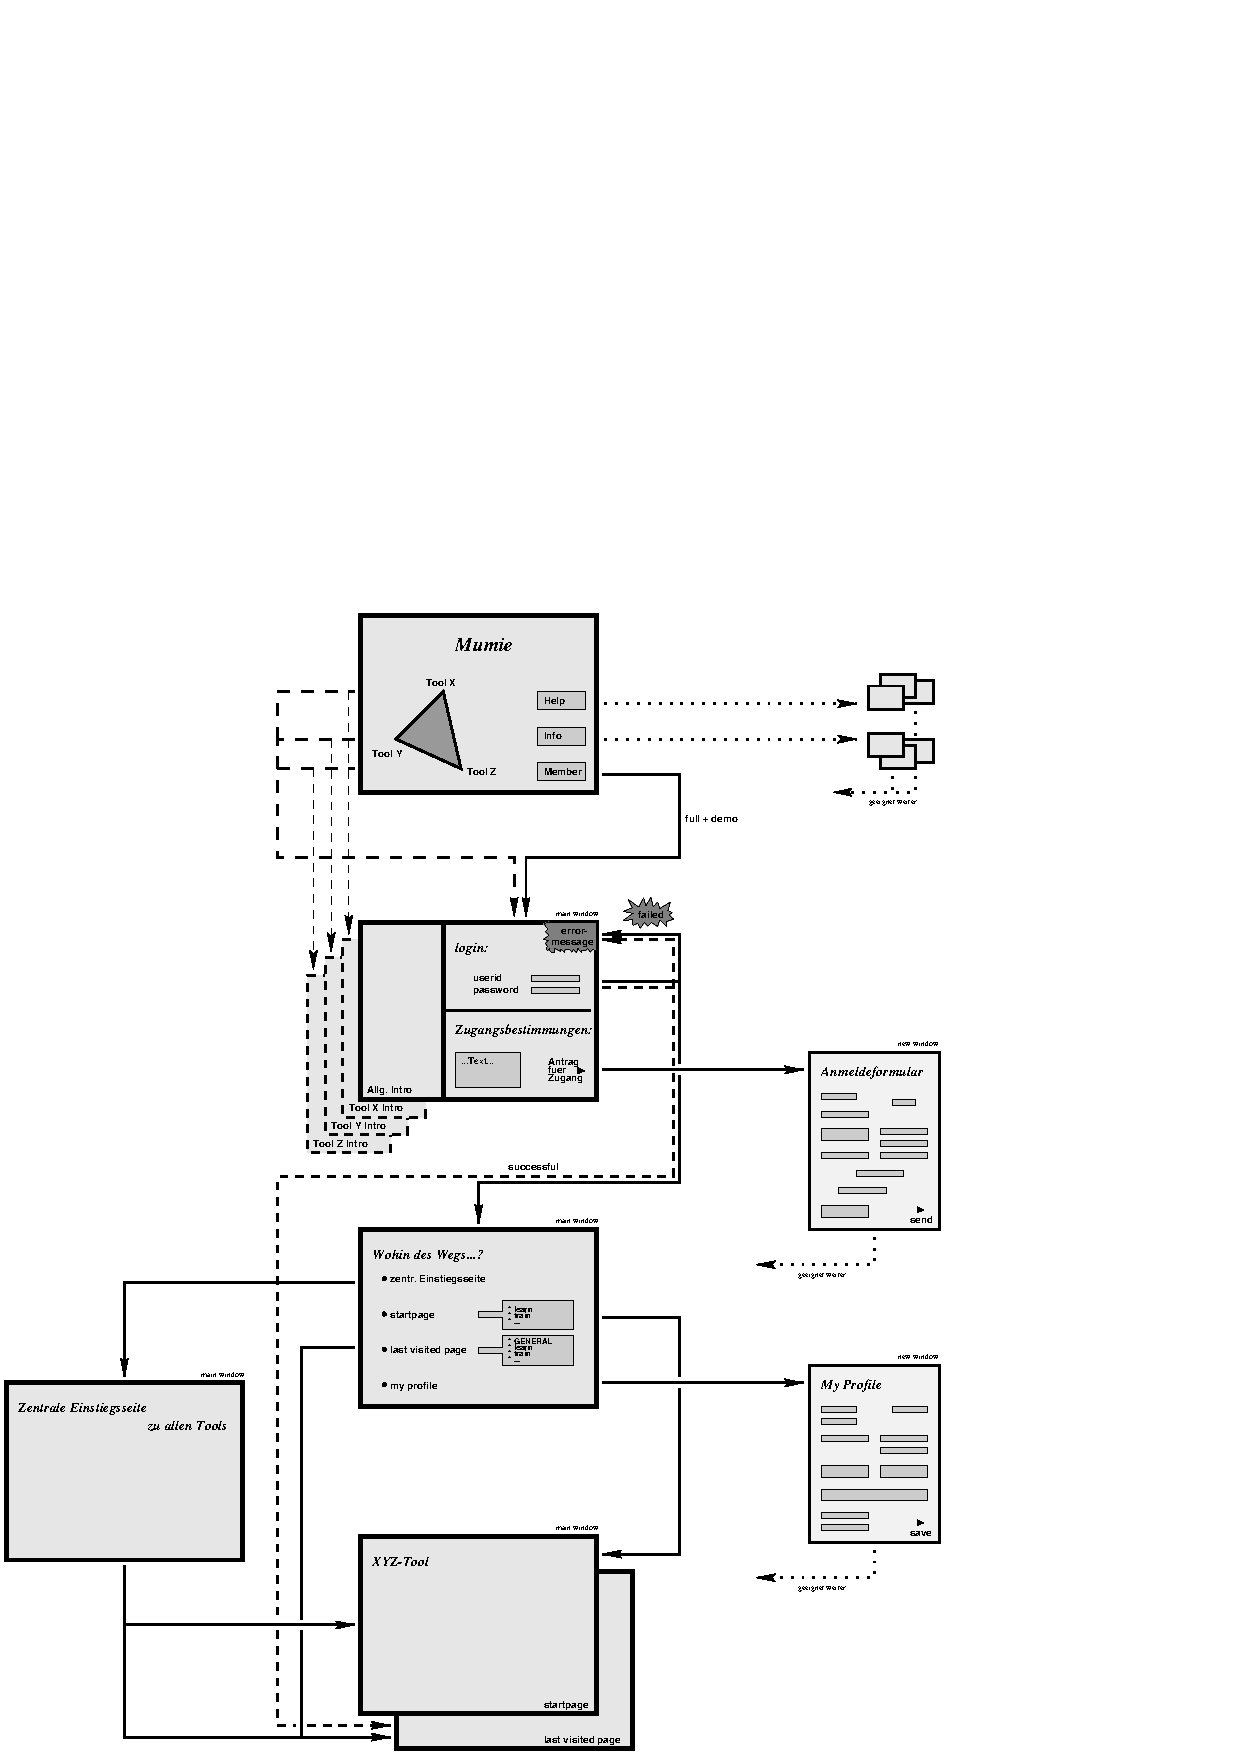
\includegraphics{Skizzen/overview_portal.pdf}
\fi
\caption{"Ubersicht "uber das Portal und die  Folgeseiten 1. und 2, Stufe}
\end{center}
\end{figure}
 













